% Springer Nature layout (for SN Computer Science). Build with: ./build.sh
% Items marked in red must be confirmed or filled in by the authors.
\documentclass[pdflatex,sn-mathphys-num]{sn-jnl}
% Packages and macros shared by both layouts.
\usepackage{amsmath,amssymb}
\usepackage{booktabs}
\usepackage{graphicx}
\usepackage{tikz}
\usetikzlibrary{arrows.meta,positioning}
\usepackage{pgfplots}
\pgfplotsset{compat=1.17}
% GENERATED by paper/scripts/make-tables.mjs from bench/results/*.json. Do not edit.
\newcommand{\EnvCpu}{Apple M1}
\newcommand{\EnvCores}{8}
\newcommand{\EnvPerfCores}{4}
\newcommand{\EnvEffCores}{4}
\newcommand{\EnvMemGb}{8}
\newcommand{\EnvMacos}{26.6.2}
\newcommand{\EnvNode}{24.10.0}
\newcommand{\EnvCircom}{2.2.3}
\newcommand{\EnvSnarkjs}{0.7.6}
\newcommand{\EnvCircomlib}{2.0.5}
\newcommand{\EnvAnchorLang}{0.30.1}
\newcommand{\EnvSolana}{3.1.13}
\newcommand{\EnvBrowser}{Chromium 156}
\newcommand{\OldConstraints}{37}
\newcommand{\NewConstraints}{339}
\newcommand{\OldWires}{39}
\newcommand{\NewWires}{341}
\newcommand{\NewWasmBytes}{1{,}750{,}062}
\newcommand{\NewWasmMb}{1.75}
\newcommand{\OldWasmKb}{36.5}
\newcommand{\NewZkeyKb}{206.9}
\newcommand{\OldZkeyKb}{22.3}
\newcommand{\NewProofBytes}{721}
\newcommand{\NewSignalsBytes}{120}
\newcommand{\UnsimplifiedConstraints}{622}
\newcommand{\UnsimplifiedLinear}{280}
\newcommand{\UnsimplifiedNonLinear}{342}
\newcommand{\PoseidonConstraints}{240}
\newcommand{\PoseidonPercent}{71}
\newcommand{\NodeRuns}{100}
\newcommand{\NodeWarmup}{5}
\newcommand{\OldFullProveMs}{30.2}
\newcommand{\NewFullProveMs}{108.4}
\newcommand{\NewWitnessMs}{30.6}
\newcommand{\NewProveMs}{74.8}
\newcommand{\OldVerifyMs}{12.3}
\newcommand{\NewVerifyMs}{13.4}
\newcommand{\ProveSlowdown}{3.6}
\newcommand{\ConstraintGrowth}{9.2}
\newcommand{\BrowserRuns}{30}
\newcommand{\BrowserWarmup}{3}
\newcommand{\BrowserProveMs}{89.4}
\newcommand{\BrowserProvePninetyfive}{101.1}
\newcommand{\NodeProvePninetyfive}{115.5}
\newcommand{\BrowserVerifyMs}{14.1}
\newcommand{\BrowserFirstProveMs}{257.1}
\newcommand{\CryptoRuns}{30}
\newcommand{\KdfIterations}{120{,}000}
\newcommand{\KdfMs}{23.3}
\newcommand{\EncSampleMs}{23.4}
\newcommand{\EncLargestMs}{27.4}
\newcommand{\SamplePlainBytes}{228}
\newcommand{\SampleStoredBytes}{451}
\newcommand{\ChainRuns}{20}
\newcommand{\AccountBytes}{212}
\newcommand{\OldAccountBytes}{180}
\newcommand{\RentLamports}{2{,}366{,}400}
\newcommand{\RentSol}{0.0023664}
\newcommand{\OldRentLamports}{2{,}143{,}680}
\newcommand{\RentIncreaseLamports}{222{,}720}
\newcommand{\TxBytes}{347}
\newcommand{\TxLimitBytes}{1{,}232}
\newcommand{\TxPercentOfLimit}{28}
\newcommand{\CuMin}{7{,}402}
\newcommand{\CuMax}{13{,}402}
\newcommand{\CuStep}{1{,}500}
\newcommand{\FeeLamports}{5{,}000}
\newcommand{\OwnerDebitLamports}{2{,}371{,}400}
\newcommand{\LocalConfirmMs}{480}
\newcommand{\CidChars}{59}


\newcommand{\papertitle}{Commitment-Bound Selective Disclosure for Patient-Held Health Records on Solana and IPFS}

% Disclosure of AI assistance. IEEE asks for it in the acknowledgments,
% Springer Nature in the methods part; each wrapper places it accordingly.
\newcommand{\aistatement}{Claude (Anthropic), a large language model used
through the Claude Code tool, assisted in this work. It was used to draft
the text of all sections of the manuscript; to implement the commitment and
challenge extension of the circuit, the client-side proving and verification
code, the test suites and the benchmark scripts; and to generate the tables
and the timing figure from the recorded measurement files. Every numerical
result reported here was obtained by executing the code on the hardware
described in Section~\ref{sec:eval}; none was produced by the model. Each
reference was checked against its publisher, standards-body or DOI registry
record. The authors reviewed the manuscript and the code and take full
responsibility for the content.}

\usepackage{xcolor}
\newif\ifspringerbuild
\springerbuildtrue
\newcommand{\tablefont}{\small}
\newcommand{\figurewidth}{0.72\textwidth}
\newcommand{\authorcheck}[1]{\textcolor{red}{[AUTHORS TO CONFIRM: #1]}}
\raggedbottom

\begin{document}

\title[Commitment-Bound Selective Disclosure for Health Records]{\papertitle}

\author*[1]{\fnm{M. Jabez Joshwin} \sur{Paul}}\email{jabezjoshwin@gmail.com}
\author[2]{\fnm{E. Bijolin} \sur{Edwin}}

\affil*[1]{\orgdiv{Division of Computer Science and Engineering},
\orgname{Karunya Institute of Technology and Sciences},
\orgaddress{\city{Coimbatore}, \state{Tamil Nadu}, \country{India}}}
\affil[2]{\orgdiv{Department of Computer Science and Engineering},
\orgname{Karunya Institute of Technology and Sciences},
\orgaddress{\city{Coimbatore}, \state{Tamil Nadu}, \country{India}}}

\abstract{\textbf{Purpose:} Patients are often asked to prove a simple fact about
their health record, such as having received at least a required number of
vaccine doses, and end up disclosing the whole record. A zero-knowledge
proof can answer the question without revealing the data, but only if the
proof is tied to a stored record and to a verification session. We address
this for a patient-held record stored on IPFS and anchored on Solana.

\textbf{Methods:} Starting from a prototype in which a server computed the
proof from the private value, we store a salted Poseidon commitment to the
value in the record's on-chain account, make the same commitment an output
of the circuit, add a verifier-chosen challenge as a public input, enforce
input ranges inside the circuit, and generate Groth16 proofs in the owner's
browser. We implement the design with Circom, snarkjs and Anchor, test it,
and measure it on a laptop.

\textbf{Results:} The bound circuit has \NewConstraints{} constraints
against \OldConstraints{} for the baseline. A proof takes a median of
\BrowserProveMs~ms to generate in a browser and \NewVerifyMs~ms to verify.
Each record occupies a \AccountBytes-byte account with a refundable deposit
of \RentSol{} SOL, and its creation consumes at most \CuMax{} compute units.

\textbf{Conclusion:} Binding a threshold proof to an on-chain commitment and
proving on the owner's device is practical for this claim. The committed
value remains self-asserted; an issuer attestation is the main missing
piece.
}

\keywords{Zero-knowledge proofs, Selective disclosure, Personal health
records, Blockchain, Solana, IPFS}

\maketitle

% Shared body of the paper. Included by main-ieee.tex and main-springer.tex.
% Numbers written as macros (\NewConstraints, ...) come from
% generated/numbers.tex, which is produced from bench/results/*.json.

\section{Introduction}\label{sec:intro}

A personal health record is a health record that the individual, rather than
a care provider, controls and shares~\cite{tang2006phr,roehrs2017phr}. Putting
the individual in control raises a practical question each time the record is
used: how much of it must be shown? Many everyday checks need only a yes-or-no
fact. A school, an employer or a border officer may need to know that a person
has received at least a required number of vaccine doses, and has no need for
the dates, the products, or the rest of the record. Handing over the whole
document to answer such a question discloses far more than the question
requires, which is at odds with the data-minimisation principle found in
data-protection law~\cite{gdpr2016}.

Blockchains have been studied extensively as a substrate for health records
because they give patients and institutions a shared, tamper-evident log
without a single operator~\cite{kuo2017blockchain,mcghin2019blockchain}. Most
proposals keep the record itself off-chain, encrypted, and use the chain to
manage pointers and permissions~\cite{azaria2016medrec,zyskind2015decentralizing,dagher2018ancile,xia2017medshare,shahnaz2019ehr,sun2020ipfs}.
In these designs the unit of sharing is still the record or a part of it: a
party that is granted access decrypts and reads the data. Zero-knowledge
proofs~\cite{goldwasser1989} offer a different unit of sharing, namely a
statement about the data, and succinct non-interactive
constructions~\cite{parno2013pinocchio,groth2016} make such statements cheap
to check.

A zero-knowledge proof about a health value is only useful to a verifier if
it is anchored to something. A proof that ``I know a number that is at least
two'' convinces nobody of anything. Three questions have to be answered by
the surrounding system: which stored record does the proof speak about, who
learned the secret while the proof was being made, and can a proof made for
one verifier be shown to another. This paper starts from a small working
prototype in which none of the three had a satisfactory answer. In that
baseline, the encrypted record was pinned to the InterPlanetary File System
(IPFS) and its content identifier was stored on Solana, but the threshold
proof was computed by a server that received the private value in clear, and
the proof contained nothing that connected it to the stored record or to a
particular verification session.

We redesign the proof path to close these gaps and measure what the redesign
costs. The contributions are as follows.
\begin{enumerate}
  \item \emph{A commitment-bound disclosure design.} A salted Poseidon
  commitment to the private value is stored in the record's on-chain account
  when the record is created, and the circuit outputs the same commitment.
  A verifier accepts a proof only if its commitment equals the one read from
  the chain. A verifier-chosen challenge is a public input of the circuit,
  which ties each proof to one verification session. Proofs are generated on
  the owner's device, so no other party sees the private value.
  \item \emph{A working implementation} on Solana (using the Anchor
  framework), IPFS, Circom and snarkjs, with automated tests for the
  circuit, the on-chain program and the client logic.
  \item \emph{A reproducible measurement} of the cost of the design on
  commodity hardware: circuit size, proving and verification time in Node.js
  and in a web browser, client-side encryption time, and on-chain storage
  and execution cost. Every figure reported here is produced by a script
  included with the implementation.
  \item \emph{An explicit account of what the design does not provide},
  including the absence of an issuer attestation, the single-party setup,
  and the information a verifier can extract by repeated queries.
\end{enumerate}

We do not claim a new cryptographic primitive. The building blocks are
standard; the contribution is their composition for this use case, an
implementation, and measurements that others can repeat.

The rest of the paper is organised as follows. Section~\ref{sec:background}
introduces the building blocks and Section~\ref{sec:related} reviews related
work. Section~\ref{sec:design} presents the threat model and the design,
Section~\ref{sec:impl} the implementation, and Section~\ref{sec:eval} the
evaluation. Section~\ref{sec:security} analyses security and limitations,
and Section~\ref{sec:conclusion} concludes.

\section{Background}\label{sec:background}

\subsection{Zero-knowledge succinct arguments}

A zero-knowledge proof lets a prover convince a verifier that a statement is
true without revealing why it is true~\cite{goldwasser1989}. A zk-SNARK is a
non-interactive argument of this kind whose proofs are short and fast to
verify. Pinocchio~\cite{parno2013pinocchio} made such arguments practical for
general computations, and Zerocash~\cite{bensasson2014zerocash} and
Hawk~\cite{kosba2016hawk} brought them to blockchains; a survey of their use
in that setting is given by Sun et al.~\cite{sun2021zkpsurvey}.

We use the pairing-based argument of Groth~\cite{groth2016}. The computation
to be proved is written as a rank-1 constraint system (R1CS) over a prime
field. A Groth16 proof consists of three group elements, and verification
checks one pairing-product equation using three pairings~\cite{groth2016}.
The scheme needs a structured reference string that is specific to the
circuit and is produced by a setup procedure; whoever knows the randomness of
that procedure can forge proofs, which is why multi-party procedures for
sampling the parameters have been developed~\cite{bensasson2015sampling}.
Our implementation works over a Barreto--Naehrig pairing-friendly
curve~\cite{barreto2006bn}, the curve that snarkjs calls \texttt{bn128}.
Alternatives that avoid a trusted setup exist, for example
Bulletproofs~\cite{bunz2018bulletproofs}, whose range proofs fit this
kind of statement at the price of larger proofs and slower verification
than Groth16.

Circuits are written in Circom~\cite{belles2023circom}, a language that
compiles a description of signals and constraints into an R1CS and a
WebAssembly witness generator. Proving and verification use
snarkjs~\cite{snarkjs}. A known hazard of this style of programming is the
\emph{under-constrained} circuit, in which the constraints admit witnesses
that the programmer did not intend, so that a malicious prover can obtain an
accepting proof for a false statement~\cite{pailoor2023underconstrained}.
This hazard shaped the range checks in Section~\ref{sec:circuit}.

\subsection{Poseidon}

Conventional hash functions such as SHA-256 are expensive to express as
arithmetic constraints. Poseidon~\cite{grassi2021poseidon} is a hash function
designed to operate natively on prime-field elements so that it needs far
fewer constraints inside a proof system. We use it as a commitment: the
commitment to a value $v$ with random salt $s$ is $C = H(v, s)$, where $H$
is Poseidon with two inputs.

\subsection{Solana accounts and program-derived addresses}

Solana stores all state in accounts. Every account has the same five fields,
among them a data buffer and an owner, and only the program that owns an
account may modify its data~\cite{solana-accounts}. An account must hold a
refundable minimum balance proportional to its size to remain on
chain~\cite{solana-accounts}. A program-derived address (PDA) is an account
address computed deterministically from a program identifier and a list of
seeds; it does not lie on the Ed25519 curve, so no private key exists for
it~\cite{solana-pda}. A transaction is limited to 1{,}232
bytes~\cite{solana-transactions}; it pays a base fee of 5{,}000 lamports per
signature, and each instruction has a default budget of 200{,}000 compute
units~\cite{solana-fees}. One SOL is $10^{9}$ lamports. Anchor is a framework
that generates account validation and serialisation code for Solana programs
from declarative annotations~\cite{anchor-docs}.

\subsection{IPFS}

IPFS is a peer-to-peer storage network in which data is addressed by a
content identifier (CID) derived from a cryptographic hash of the data
itself~\cite{benet2014ipfs,trautwein2022ipfs}. Because the address is a
function of the content, anyone who retrieves the data can check that it has
not been altered. Content remains retrievable only while some node keeps it;
\emph{pinning} services keep content on behalf of
users~\cite{daniel2022ipfs}. IPFS provides no confidentiality: anyone who
knows a CID can request the content, so private data must be encrypted
before it is added.

\subsection{Password-based authenticated encryption}

AES in Galois/Counter Mode (GCM) is an authenticated encryption mode; NIST
recommends a 96-bit initialisation vector for it~\cite{dworkin2007gcm}.
PBKDF2 derives a symmetric key from a passphrase by iterating a pseudorandom
function over the passphrase and a salt~\cite{rfc8018,turan2010pbkdf}. Both
are available in browsers through the Web Cryptography
API~\cite{w3c2017webcrypto}. The iteration count determines the cost of each
passphrase guess; NIST SP~800-132 asks for a count as large as is
feasible~\cite{turan2010pbkdf}, and current OWASP guidance recommends
600{,}000 iterations for PBKDF2 with HMAC-SHA-256~\cite{owasp-password}.

\section{Related Work}\label{sec:related}

\paragraph{Blockchain-based health record management}
Zyskind et al.~\cite{zyskind2015decentralizing} proposed keeping personal
data off-chain and using a blockchain as an access-control manager.
MedRec~\cite{azaria2016medrec} applied the idea to medical records, using
smart contracts to manage permissions over records that remain with
providers. Yue et al.~\cite{yue2016hdg} described a gateway application that
lets patients own and control their data. Ancile~\cite{dagher2018ancile}
combines smart contracts with further cryptographic techniques for access
control and interoperability, and MeDShare~\cite{xia2017medshare} records
data-sharing actions among cloud custodians on a blockchain to provide
provenance and auditing. FHIRChain~\cite{zhang2018fhirchain} builds a
blockchain-based architecture around the HL7 FHIR standard for sharing
clinical data. Shahnaz et al.~\cite{shahnaz2019ehr} and Tanwar et
al.~\cite{tanwar2020ehr} present frameworks for electronic health records
with access rules enforced on a blockchain. Sun et al.~\cite{sun2020ipfs}
store encrypted medical records in IPFS and control access with
ciphertext-policy attribute-based encryption. Surveys of the area
identify privacy, scalability and regulatory compliance as open
challenges~\cite{kuo2017blockchain,mcghin2019blockchain,zhang2020security}.

These systems answer the question of \emph{who may read a record}. Once
access is granted, the reader obtains the data. Our work addresses a
complementary question, namely how an owner can let a verifier check a
predicate over a record without granting read access at all.

\paragraph{Zero-knowledge proofs and credentials in health applications}
Sharma et al.~\cite{sharma2020zkp} combine zero-knowledge proofs with proxy
re-encryption in a blockchain framework for managing access to health records
and funds. Selective disclosure has a long history in anonymous credential
systems~\cite{camenisch2001credentials}, and the W3C Verifiable Credentials
data model~\cite{w3c2025vc} standardises a format for issuer-signed
credentials in which a holder can choose what to disclose, including through
zero-knowledge mechanisms. Those systems rest on an issuer who signs the
attributes. Our prototype has no issuer; the on-chain commitment fixes a
value at a point in time but does not attest that the value is true. We
return to this limitation in Section~\ref{sec:limits}.

\paragraph{Positioning}
We are not aware of a published measurement of a commitment-bound threshold
proof for health records on Solana with client-side proving, but we have not
carried out a systematic review and make no claim of being first. We do not
compare our measurements numerically with the systems above: they run on
different ledgers, solve different problems and report different metrics, so
a side-by-side table of numbers would not be meaningful.

\section{System Design}\label{sec:design}

\subsection{Roles and threat model}\label{sec:threat}

The system has three roles. The \emph{owner} holds a health record and a
wallet key. A \emph{verifier} wants to know whether a numeric field of the
record, here the vaccination count, is at least some threshold. The
\emph{infrastructure} consists of the Solana ledger, the IPFS network with a
pinning service, and a web server that delivers the application code.

We consider the following adversaries.
\begin{itemize}
  \item \emph{Chain and storage observers.} Everything written to Solana
  and to IPFS is public and permanent for practical purposes. Observers try
  to learn the contents of records from it.
  \item \emph{A curious verifier.} The verifier follows the protocol but
  tries to learn more than the truth of the predicate.
  \item \emph{A dishonest prover.} A party tries to make a verifier accept a
  statement that is false for the record at a given address, or to reuse a
  proof it obtained from someone else.
  \item \emph{A curious service operator.} The operators of the pinning
  service and of any auxiliary server try to learn private values from what
  passes through them.
\end{itemize}

We assume that the owner's device and browser are not compromised, that the
application code and the verification key reach each party unmodified, that
the setup of the proof system was honest, and that the cryptographic
primitives are secure. The owner is \emph{not} assumed to be truthful about
the data: the design makes no claim that the committed value is medically
correct. Denial of service is out of scope.

\subsection{Design goals}

\begin{itemize}
  \item \emph{G1, record confidentiality.} Observers and operators learn
  nothing about a record's contents beyond its size.
  \item \emph{G2, minimal disclosure.} From an accepted proof a verifier
  learns that the count is at least the threshold and nothing else about the
  count.
  \item \emph{G3, binding to a record.} An accepted proof is about the value
  that was committed when the record at the stated address was created.
  \item \emph{G4, session freshness.} A proof made for one challenge is not
  accepted for another.
  \item \emph{G5, local proving.} No party other than the owner's device
  handles the private value or the salt in clear.
\end{itemize}

\subsection{Architecture}

\begin{figure}[t]
\centering
% Architecture and data flow (TikZ). Sized to fit one IEEE column.
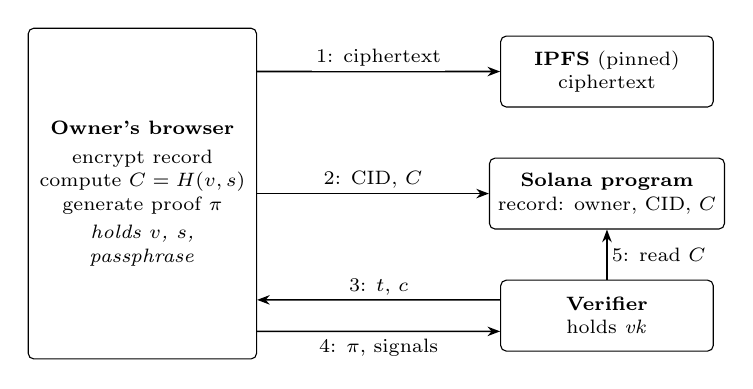
\begin{tikzpicture}[
  font=\fontsize{7}{8.4}\selectfont,
  box/.style={draw, rounded corners=2pt, align=center, inner sep=3pt, minimum height=9mm},
  flow/.style={-{Stealth[length=1.6mm]}, semithick},
  lab/.style={font=\fontsize{7}{8.4}\selectfont, align=center, inner sep=1.5pt, fill=white},
]
  \node[box, minimum width=29mm, minimum height=42mm, align=center] (owner) at (0,0)
    {\textbf{Owner's browser}\\[2pt]encrypt record\\compute $C=H(v,s)$\\generate proof $\pi$\\[2pt]\emph{holds $v$, $s$,}\\\emph{passphrase}};
  \node[box, minimum width=27mm] (ipfs) at (5.9,1.55)
    {\textbf{IPFS} (pinned)\\ciphertext};
  \node[box, minimum width=27mm] (chain) at (5.9,0)
    {\textbf{Solana program}\\record: owner, CID, $C$};
  \node[box, minimum width=27mm] (verifier) at (5.9,-1.55)
    {\textbf{Verifier}\\holds $\mathit{vk}$};

  \draw[flow] ([yshift=1.55cm]owner.east) -- node[lab, above] {1: ciphertext} (ipfs.west);
  \draw[flow] ([yshift=0cm]owner.east) -- node[lab, above] {2: CID, $C$} (chain.west);
  \draw[flow] ([yshift=2mm]verifier.west) -- node[lab, above] {3: $t$, $c$} ([yshift=-1.35cm]owner.east);
  \draw[flow] ([yshift=-1.75cm]owner.east) -- node[lab, below, yshift=-1pt] {4: $\pi$, signals} ([yshift=-2mm]verifier.west);
  \draw[flow] (verifier.north) -- node[lab, right] {5: read $C$} (chain.south);
\end{tikzpicture}

\caption{Architecture and data flow. Steps 1--2 create a record; steps 3--5
are one disclosure. Step 4 carries the record address, the proof $\pi$ and
the public signals. The private count and salt never leave the owner's
browser.}
\label{fig:arch}
\end{figure}

Figure~\ref{fig:arch} shows the components. The owner's browser performs all
operations on private data: encryption, commitment and proving. The pinning
service receives only ciphertext, through a server-side route that holds the
service credential. The Solana program stores one small account per record.
The verifier needs only the verification key, read access to the chain, and
the proof.

\subsection{Record creation}

Let $v$ be the private count. To create a record the owner's browser
\begin{enumerate}
  \item samples a salt $s$ of 248 random bits and stores it as a field of
  the record;
  \item computes the commitment $C = H(v, s)$;
  \item derives a 256-bit key from the owner's passphrase with PBKDF2 and a
  fresh 128-bit salt, encrypts the record (including $s$) with AES-256-GCM
  under a fresh 96-bit initialisation vector, and uploads the result to
  IPFS, obtaining a CID;
  \item sends an \texttt{init\_record} transaction that creates the record
  account and stores the owner's public key, the CID, a client-supplied
  timestamp and $C$.
\end{enumerate}
The account address is a PDA derived from the seeds
(\texttt{"record"}, owner key, timestamp), so each upload creates a new
account and existing accounts are never overwritten. The program stores $C$
as 32 opaque bytes; it neither interprets nor checks it. Keeping the salt
inside the encrypted record means that the owner needs only the passphrase
to prove again later from any device.

\subsection{Disclosure protocol}\label{sec:protocol}

A disclosure involves the following steps.
\begin{enumerate}
  \item The verifier chooses a threshold $t$ and a fresh random challenge
  $c$, and sends both to the owner.
  \item The owner's browser generates a Groth16 proof $\pi$ for the relation
  in Section~\ref{sec:circuit} with private inputs $(v, s)$ and public inputs
  $(t, c)$, and sends the verifier the record address, $\pi$ and the public
  signals $(b, C', t', c')$.
  \item The verifier reads the commitment $C$ from the record account at
  that address, directly from a Solana node.
  \item The verifier accepts if and only if
  \begin{equation}\label{eq:accept}
  \begin{gathered}
    C' = C,\qquad t' = t,\qquad c' = c,\qquad b = 1,\\
    \mathsf{Verify}\bigl(\mathit{vk},\,(b, C', t', c'),\,\pi\bigr) = 1 .
  \end{gathered}
  \end{equation}
\end{enumerate}
The verifier never takes the commitment from the prover's message as given;
it is compared with the on-chain value. Each failed condition yields a
distinct rejection reason in the implementation, which makes misuse easier
to diagnose.

\subsection{The circuit}\label{sec:circuit}

Let $\mathbb{F}_p$ be the scalar field of the curve and $n = 32$. The circuit
enforces the relation
\begin{equation}\label{eq:relation}
\begin{aligned}
  \mathcal{R} = \bigl\{\, &((b, C, t, c),\,(v, s)) \;:\; v, t \in [0, 2^{n}),\\
  & C = H(v, s),\;\; b = 1 \text{ if } v \ge t,\;\; b = 0 \text{ otherwise} \,\bigr\}
\end{aligned}
\end{equation}
with $(v, s)$ private and $(b, C, t, c)$ public. The comparison is computed
as $t < v + 1$ with a comparator on $n + 1$ bits, because $v + 1$ can reach
$2^{n}$.

Two details matter for soundness. First, the comparator from the Circom
standard library is correct only when both operands fit in the stated number
of bits. The baseline circuit relied on that precondition without enforcing
it. The new circuit decomposes $v$ and $t$ into $n$ bits each, so the bound
is part of the proved statement rather than an assumption about the prover.
Second, the challenge $c$ does not take part in the predicate, and a public
input that appears in no constraint may not be bound by the proof. The
circuit therefore includes one multiplication constraint, $c \cdot c$, whose
only purpose is to tie $c$ into the constraint system.

The bit $b$ is an output rather than a hard constraint. A proof with $b = 0$
is a valid proof that the count is \emph{below} the threshold; the
verifier's rule~\eqref{eq:accept} requires $b = 1$.

\section{Implementation}\label{sec:impl}

The prototype has four parts.

\paragraph{Circuit} The circuit is about fifty lines of Circom and uses the
bit-decomposition, comparator and Poseidon templates of circomlib. It is
compiled with full constraint simplification. The proving and verification
keys come from a single-contributor setup run with snarkjs
(Section~\ref{sec:limits}).

\paragraph{On-chain program} The program is written in Rust with Anchor
\EnvAnchorLang. It has one instruction, \texttt{init\_record}, and one
account type holding the owner key (32 bytes), the CID as a string of at
most 128 bytes, a 64-bit timestamp and the 32-byte commitment. With Anchor's
8-byte type discriminator and the 4-byte string length prefix the account
occupies \AccountBytes{} bytes. A CID longer than 128 bytes is rejected with
a dedicated error. The owner must sign and pays for the account.

\paragraph{Client} The web client is a Next.js application. It uses the Web
Cryptography API for PBKDF2 (HMAC-SHA-256, \KdfIterations{} iterations) and
AES-256-GCM, and loads snarkjs, the WebAssembly witness generator
(\NewWasmMb~MB) and the proving key (\NewZkeyKb~kB) to prove in the browser.
The commitment is computed outside the circuit with an independent Poseidon
implementation, and a test checks that the two agree. The client contains an
owner view, which creates records and generates proofs, and a verifier view,
which reads a record account by address and applies rule~\eqref{eq:accept}.
The verifier view needs no wallet.

\paragraph{Auxiliary services} Uploads to the pinning service pass through
a server-side route that holds the service credential; it sees ciphertext
only. A small optional HTTP service verifies a proof against the
verification key for clients that cannot run snarkjs. Unlike the baseline's
proof service, it never receives private inputs.

\ifspringerbuild
\paragraph{Development method and use of AI tools} \aistatement
\fi

\section{Evaluation}\label{sec:eval}

The evaluation answers three questions. What does binding the proof to the
record cost in circuit size and time? Is proving on the owner's device
practical? What does a record cost on chain?

\subsection{Setup and method}

All measurements were taken on one laptop: an \EnvCpu{} system with
\EnvCores{} cores (\EnvPerfCores{} performance and \EnvEffCores{}
efficiency) and \EnvMemGb~GB of memory, running macOS \EnvMacos. Software
versions were Node.js \EnvNode, Circom \EnvCircom, circomlib \EnvCircomlib,
snarkjs \EnvSnarkjs, Anchor \EnvAnchorLang{} and the Solana tool suite
\EnvSolana.

We compare two circuits. \emph{Baseline} is the threshold-only circuit of
the original prototype, with one private input and no commitment, challenge
or range checks. \emph{Bound} is the circuit of Section~\ref{sec:circuit}.
Timings in Node.js are wall-clock times over \NodeRuns{} runs after
\NodeWarmup{} unmeasured warm-up runs. Browser timings were taken in
\EnvBrowser{} on the same machine with a production build of the client,
over \BrowserRuns{} runs after \BrowserWarmup{} warm-up runs. Encryption
timings use the client's own encryption functions over \CryptoRuns{} runs.
On-chain costs were measured on a local Solana test validator with the
program loaded, over \ChainRuns{} transactions with a \CidChars-character
CID. We report medians with the 5th and 95th percentiles.

We did not measure confirmation latency on a public Solana cluster or upload
latency to a pinning service; both depend on network conditions and on
third-party services, and the numbers below should not be read as including
them.

\subsection{Circuit size}

\begin{table}[t]
\centering
\caption{Size of the constraint system and of the artifacts.}
\label{tab:circuit}
\tablefont
% GENERATED by paper/scripts/make-tables.mjs. Do not edit.
\begin{tabular}{@{}lrr@{}}
\toprule
Quantity & Baseline & Bound \\
\midrule
R1CS constraints & 37 & 339 \\
Wires & 39 & 341 \\
Private inputs & 1 & 2 \\
Public signals & 2 & 4 \\
\midrule
Witness generator (bytes) & 36{,}469 & 1{,}750{,}062 \\
Proving key (bytes) & 22{,}333 & 206{,}869 \\
Verification key, JSON (bytes) & 3{,}109 & 3{,}476 \\
Proof, JSON (bytes) & 721 & 721 \\
Public signals, JSON (bytes) & 9 & 120 \\
\bottomrule
\end{tabular}

\end{table}

Table~\ref{tab:circuit} compares the two circuits. Binding raises the number
of constraints from \OldConstraints{} to \NewConstraints, a factor of
\ConstraintGrowth. Most of the increase comes from the commitment: a
circuit containing only the two-input Poseidon hash compiles to
\PoseidonConstraints{} constraints, about \PoseidonPercent\% of the total.
The range checks and the wider comparator account for most of the rest.
Compiler
simplification matters: without it the same circuit has
\UnsimplifiedConstraints{} constraints, of which \UnsimplifiedLinear{} are
linear and are eliminated by simplification.

The proof is the same size in both cases, as expected for Groth16, whose
proofs always consist of three group elements~\cite{groth2016}; its JSON
encoding is \NewProofBytes{} bytes. The public signals grow because they now
include the commitment and the challenge. The artifact that grows most is
the witness generator, from \OldWasmKb~kB to \NewWasmMb~MB, because it embeds
the Poseidon round constants. This is a one-time download for the owner's
browser and can be cached.

\subsection{Proving and verification time}

\begin{table}[t]
\centering
\caption{Time in milliseconds: median (5th--95th percentile).}
\label{tab:timing}
\tablefont
% GENERATED by paper/scripts/make-tables.mjs. Do not edit.
\begin{tabular}{@{}lrr@{}}
\toprule
Operation & Baseline & Bound \\
\midrule
\multicolumn{3}{@{}l}{\emph{Node.js, $n=100$}} \\
Witness generation & 5.3 (4.4--6.2) & 30.6 (30.1--31.3) \\
Groth16 proving & 22.9 (20.1--26.1) & 74.8 (67.9--78.9) \\
Witness + proving & 30.2 (28.8--32.9) & 108.4 (103.4--115.5) \\
Verification & 12.3 (12.1--14.0) & 13.4 (13.2--13.8) \\
\midrule
\multicolumn{3}{@{}l}{\emph{Browser (Chromium 156), $n=30$}} \\
Witness + proving & --- & 89.4 (82.8--101.1) \\
Verifier check & --- & 14.1 (13.6--15.0) \\
\bottomrule
\end{tabular}

\end{table}

\begin{figure}[t]
\centering
% Timing bar chart (pgfplots). Data are generated from bench/results.
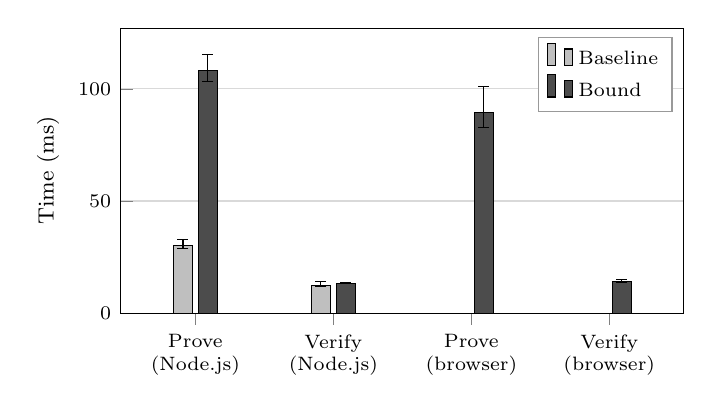
\begin{tikzpicture}
\begin{axis}[
  ybar,
  width=\figurewidth,
  height=5.2cm,
  bar width=7pt,
  ymin=0,
  ylabel={Time (ms)},
  ylabel style={font=\footnotesize},
  symbolic x coords={PN,VN,PB,VB},
  xtick={PN,VN,PB,VB},
  xtick pos=bottom,
  ytick pos=left,
  xticklabels={{Prove\\(Node.js)},{Verify\\(Node.js)},{Prove\\(browser)},{Verify\\(browser)}},
  xticklabel style={font=\scriptsize, align=center},
  yticklabel style={font=\scriptsize},
  enlarge x limits=0.18,
  ymajorgrids,
  grid style={black!15},
  legend style={font=\scriptsize, at={(0.98,0.97)}, anchor=north east, draw=black!40},
  legend cell align=left,
  cycle list={},
]
% GENERATED by paper/scripts/make-tables.mjs. Do not edit.
\addplot+[fill=black!25, draw=black, error bars/.cd, y dir=both, y explicit] coordinates {(PN,30.226) += (0,2.624) -= (0,1.452) (VN,12.297) += (0,1.733) -= (0,0.241)};
\addplot+[fill=black!70, draw=black, error bars/.cd, y dir=both, y explicit] coordinates {(PN,108.384) += (0,7.128) -= (0,4.946) (VN,13.41) += (0,0.417) -= (0,0.227) (PB,89.4) += (0,11.665) -= (0,6.605) (VB,14.1) += (0,0.875) -= (0,0.455)};

\legend{Baseline, Bound}
\end{axis}
\end{tikzpicture}

\caption{Median proving and verification time. Whiskers show the 5th and
95th percentiles. The baseline was not run in the browser because it proved
on a server.}
\label{fig:timing}
\end{figure}

Table~\ref{tab:timing} and Fig.~\ref{fig:timing} give the timings. In
Node.js, witness generation plus proving takes \NewFullProveMs~ms for the
bound circuit against \OldFullProveMs~ms for the baseline, a factor of
\ProveSlowdown{} for \ConstraintGrowth{} times as many constraints.
Verification time is practically unchanged, \NewVerifyMs~ms against
\OldVerifyMs~ms, because Groth16 verification cost depends on the number of
public inputs and not on the size of the circuit.

In the browser, the complete proving step has a median of
\BrowserProveMs~ms and a 95th percentile of \BrowserProvePninetyfive~ms once
the artifacts are loaded. The first proof after a page load took
\BrowserFirstProveMs~ms in our run, which includes fetching and compiling the
witness generator. The verifier's complete check, including the comparisons
of rule~\eqref{eq:accept}, has a median of \BrowserVerifyMs~ms. For this
circuit, proving on the owner's device is therefore well within interactive
latency on a laptop, and the server-side prover of the baseline is not
needed for performance reasons. We did not measure phones or low-end
devices, where proving will be slower.

\subsection{Client-side encryption}

\begin{table}[t]
\centering
\caption{Client-side encryption and decryption (median, ms). ``Stored'' is
the size of the JSON object pinned to IPFS.}
\label{tab:crypto}
\tablefont
% GENERATED by paper/scripts/make-tables.mjs. Do not edit.
\begin{tabular}{@{}rrrr@{}}
\toprule
Plaintext & Stored & Encrypt & Decrypt \\
(bytes) & (bytes) & (ms) & (ms) \\
\midrule
228 & 451 & 23.4 & 23.4 \\
1{,}024 & 1{,}511 & 23.5 & 23.4 \\
16{,}384 & 21{,}991 & 23.7 & 23.6 \\
65{,}536 & 87{,}527 & 24.6 & 23.8 \\
262{,}144 & 349{,}671 & 27.4 & 24.8 \\
\bottomrule
\end{tabular}

\end{table}

Table~\ref{tab:crypto} shows encryption and decryption times for records of
increasing size. Key derivation alone takes \KdfMs~ms and dominates: the
sample record encrypts in \EncSampleMs~ms and a record of 256~KiB in
\EncLargestMs~ms. The stored object is larger than the plaintext because the
ciphertext is Base64-encoded and wrapped with its salt, initialisation vector
and algorithm labels; the sample record of \SamplePlainBytes{} bytes becomes
\SampleStoredBytes{} bytes.

That key derivation takes only about 23~ms is not purely good news. The same
cost applies to each guess of an attacker who downloads the public
ciphertext, and the configured \KdfIterations{} iterations are below the
600{,}000 that OWASP currently recommends for this
function~\cite{owasp-password}. We discuss this in
Section~\ref{sec:limits}.

\subsection{On-chain cost}

\begin{table}[t]
\centering
\caption{On-chain cost of creating one record (local test validator).}
\label{tab:chain}
\tablefont
% GENERATED by paper/scripts/make-tables.mjs. Do not edit.
\begin{tabular}{@{}lr@{}}
\toprule
Quantity & Value \\
\midrule
Record account size (bytes) & 212 \\
Rent-exempt deposit (lamports) & 2{,}366{,}400 \\
Transaction size (bytes) & 347 \\
Compute units consumed & 7{,}402--13{,}402 \\
Transaction fee (lamports) & 5{,}000 \\
Total debit to owner (lamports) & 2{,}371{,}400 \\
\bottomrule
\end{tabular}

\end{table}

Table~\ref{tab:chain} lists the cost of \texttt{init\_record}. The record
account occupies \AccountBytes{} bytes, 32 more than in the baseline, and
requires a refundable deposit of \RentLamports{} lamports (\RentSol{} SOL).
This matches the documented formula for the minimum
balance~\cite{solana-accounts}. Storing the commitment adds
\RentIncreaseLamports{} lamports to the deposit compared with the baseline
layout. The transaction is \TxBytes{} bytes, \TxPercentOfLimit\% of the
1{,}232-byte limit~\cite{solana-transactions}, and pays the base fee of
\FeeLamports{} lamports for its single signature.

The instruction consumed between \CuMin{} and \CuMax{} compute units, far
below the default budget of 200{,}000~\cite{solana-fees}. The observed values
differ by exact multiples of \CuStep{} units. We attribute this to the search
for the PDA bump seed, which depends on the owner key and timestamp and
therefore varies between records; we did not instrument the runtime to
confirm the attribution. On the local validator a transaction reached the
\emph{confirmed} commitment level in a median of \LocalConfirmMs~ms; this
figure describes the test setup only.

The on-chain cost is independent of the size of the health record, since the
chain stores only the CID and the commitment. Proof verification costs
nothing on chain because it happens off chain.

\subsection{Functional validation}

The implementation has 28 automated tests. Eleven exercise the circuit:
correct outputs above, at and below the threshold; the largest 32-bit
values; agreement of the in-circuit commitment with an independent Poseidon
implementation; rejection of out-of-range inputs at witness generation; and
rejection of proofs whose public commitment, challenge or validity bit has
been altered. Six run the program on a local validator: correct storage of
all fields, the exact account size, acceptance of a 128-byte CID and
rejection of a 129-byte one, rejection of a duplicate record, and rejection
of a record whose stated owner did not sign. Eleven cover the client logic,
including each rejection reason of rule~\eqref{eq:accept}. In addition, the
verifier view was exercised interactively in a browser against a record on
the local validator: a matching proof was accepted, and the same proof was rejected
after changing the expected challenge and after raising the expected
threshold. The upload path was tested through the program's client library;
the wallet extension's signing dialogue in the browser is not covered by
automated tests.

\section{Security Analysis and Limitations}\label{sec:security}

\subsection{How the goals are met}

The arguments in this subsection are informal and rest on the assumptions of
Section~\ref{sec:threat}.

\emph{G1, record confidentiality.} Only the AES-GCM ciphertext, its salt and
its initialisation vector are stored on IPFS, and only the CID and the
commitment are stored on chain. Each record is encrypted under a key derived
with a fresh salt, so an initialisation vector is never reused under the
same key. Confidentiality reduces to the security of AES-GCM and to the
strength of the passphrase.

\emph{G2, minimal disclosure.} Groth16 is zero-knowledge~\cite{groth2016},
so the proof reveals nothing beyond the public signals $(b, C, t, c)$. The
threshold and challenge were chosen by the verifier. The commitment
$C = H(v, s)$ is already public on chain; the count has very few plausible
values, so without a salt it could be recovered by trying each one, and the
248-bit random salt prevents this. We treat $H(v, \cdot)$ with a uniformly
random second input as hiding $v$, which is a heuristic assumption about
Poseidon and not a proved property.

\emph{G3, binding to a record.} If the verifier accepts, then by the
knowledge soundness of Groth16 the prover knows $(v, s)$ with $H(v, s) = C$
and $v \ge t$, where $C$ is the value read from the chain. The record
account cannot be modified after creation, since the program has no
instruction that writes to an existing account. Finding a second opening
$(v', s')$ of the same commitment with $v' \ne v$ would be a collision in
Poseidon. The proof is therefore about the value committed at creation time.
The range checks close the under-constrained comparison discussed in
Section~\ref{sec:circuit}.

\emph{G4, session freshness.} The challenge is a public input, so a proof
verifies only together with the challenge it was made for. A verifier that
draws a fresh challenge for each session will reject a proof recorded in an
earlier session. Tests confirm that altering the challenge, the commitment
or the validity bit of a genuine proof makes verification fail.

\emph{G5, local proving.} Witness generation and proving run in the owner's
browser. The verification service and the pinning route receive no private
input.

\subsection{Limitations}\label{sec:limits}

We list the limitations of the design and of the prototype in what we judge
to be decreasing order of importance.

\emph{The data is self-asserted.} Nothing prevents an owner from committing
to a count that is false. The system proves consistency with a value fixed
in the past, not correctness of that value. A deployment would need an
issuer, such as a clinic, to sign the commitment or the underlying
attributes, with the signature checked by the verifier or inside the
circuit, as in credential
systems~\cite{camenisch2001credentials,w3c2025vc}.

\emph{The proof is not bound to the presenter.} Anyone who knows $(v, s)$
can prove. The challenge stops later replay but not a relay in which an
intermediary forwards a verifier's challenge to the real owner and passes
the answer back as its own. Since the record account names the owner's
public key, the verifier could additionally require a signature on the
challenge under that key; the prototype does not do this.

\emph{Repeated queries leak the value.} Each accepted or rejected proof
tells the verifier one bit. A verifier, or several colluding verifiers, who
obtain answers for different thresholds can narrow down the count, in the
worst case exactly. The owner decides which requests to answer, but the
prototype offers no policy support for this.

\emph{Single-party setup.} The proving key was generated by one contributor
on a development machine. Anyone who retained the setup randomness could
forge proofs. A real deployment needs a multi-party
ceremony~\cite{bensasson2015sampling} or a proof system without a trusted
setup~\cite{bunz2018bulletproofs}.

\emph{Passphrase-based encryption of public ciphertext.} The ciphertext is
public and cannot be recalled, so an attacker can test passphrases offline
without limit. The configured iteration count is below current
guidance~\cite{owasp-password}, and a leaked passphrase compromises the
record permanently. A memory-hard key derivation function or a key held by
the wallet would be stronger.

\emph{Linkability and metadata.} Records are linked to the owner's wallet
address, and their creation times and number are public. All proofs about
one record carry the same commitment and are therefore linkable to each
other and to that record.

\emph{No revocation or erasure.} The program cannot update or close a
record, and content on IPFS persists while any node keeps it. This conflicts
with a right to erasure such as that of Article~17 of the
GDPR~\cite{gdpr2016} if the ciphertext or the commitment is considered
personal data, a question we do not resolve here.

\emph{Off-chain verification.} Proofs are verified by the verifier's own
software. The verifier must obtain the correct verification key through a
channel it trusts; the prototype serves it with the application. The
timestamp in a record is supplied by the client and is not checked against
the cluster clock.

\emph{Scope of the evaluation.} One claim type, one machine, a local
validator, no public-cluster or pinning-service latency, no mobile devices
and no user study.

\subsection{Future work}

The most valuable extension is issuer attestation, which would turn the
self-asserted commitment into a credential. Binding proofs to the owner's
wallet key, a multi-party setup, and anchoring a hash of the verification
key on chain address the next three limitations. The circuit generalises
directly to other numeric predicates and to several attributes committed
together; measuring how proving time grows with the number of attributes on
phones is the natural next experiment. Verifying the proof inside the Solana
program would let other programs act on a disclosure, at a compute cost that
remains to be measured.

\section{Conclusion}\label{sec:conclusion}

A zero-knowledge proof about a health record is only as meaningful as its
connection to a stored record and to a verification session. Starting from a
prototype that lacked both connections and revealed the private value to a
server, we added a salted Poseidon commitment stored on Solana, a
verifier-chosen challenge, enforced range checks and client-side proving.
On a laptop the resulting circuit has \NewConstraints{} constraints, proves
in about \BrowserProveMs~ms in a browser and verifies in about
\NewVerifyMs~ms, and each record costs a \AccountBytes-byte account with a
refundable deposit of \RentSol{} SOL. The design gives a verifier a
yes-or-no answer about a committed value without access to the record. It
does not establish that the committed value is true, and we have set out
that and the other limitations that stand between this prototype and a
deployable system.


\backmatter

\section*{Declarations}

\bmhead{Funding} \authorcheck{state the funding source, or that no funding
was received.}

\bmhead{Competing interests} \authorcheck{state any competing interests, or
that the authors have none to declare.}

\bmhead{Ethics approval} This work uses synthetic sample data only. No human
participants, patient data or animals were involved.

\bmhead{Data and code availability} The source code, the test suites, the
benchmark scripts and the recorded measurement files from which every table
and figure in this article is generated are in the project repository.
\authorcheck{give the public repository address and the commit that matches
this manuscript.}

\bmhead{Author contributions} \authorcheck{describe each author's
contribution.}

% The class selects the sn-mathphys-num reference style itself.
\bibliography{refs}

\end{document}
